\documentclass[10pt]{article}
\usepackage[margin=0.9in]{geometry}
\usepackage{amsmath,amssymb}
\usepackage[T1]{fontenc}
\usepackage[utf8]{inputenc}
\usepackage{lmodern}
\usepackage{microtype}
\usepackage{booktabs}
\usepackage{enumitem}
\usepackage{graphicx}
\usepackage[hidelinks]{hyperref}
\hypersetup{pdftitle={The Herschel Mirror as a Dish Antenna: An Archival Total-Power Search for a 541.7 GHz Line}}
\setlist{nosep,leftmargin=1.3em}
\setlength{\parskip}{4pt}\setlength{\parindent}{0pt}
\sloppy
\begin{document}
\begin{center}
{\Large\bfseries The Herschel Mirror as a Dish Antenna:\\ An Archival Total-Power Search for a 541.7\,GHz Line}\\[6pt]
{\small Working note, 2026-10-15, v1.1 (note added: the 541.700\,GHz hint is instrumental). AI-assisted research programme; not peer reviewed.}
\end{center}

\begin{abstract}\noindent
A flat or curved conductor immersed in a kinetically mixed vector field of mass $m$ radiates photons of energy $mc^2$. We used the 3.5\,m primary mirror of the Herschel Space Observatory as such a dish antenna, with archival HIFI band-1a heterodyne data as the receiver.

\textbf{Target.} We searched at 541.664\,GHz ($m=2.240$\,meV). This is the only vacuum-induced quantum mass of a gravity framework that ties the galactic acceleration scale to the dark-energy density.

\textbf{The method.} A mirror-generated line cancels in the archived (reference-subtracted) spectra, because both chop phases view the sky through the primary. We therefore rebuilt total-power spectra from raw Level-0 counts against Herschel's internal hot and cold loads. A real line must sit at a fixed spacecraft-frame frequency in every observation, whatever the target.

\textbf{Result.} From 49 observations (7.0\,h; 150 spectra), we find no line: $a=-6.7\pm7.7$\,mK (DSB peak), $z=-0.86$. The 95\% upper limit is 12.7\,mK. This gives $\varepsilon<1.9\times10^{-11}$ for a dish-coupling factor $S=50$ (range $8.6\times10^{-12}$ to $8.6\times10^{-11}$ for $S=10$ to $1000$). All four pre-registered controls pass, and a mutation test recovers an injected line at $9\sigma$.

\textbf{What it closes.} The bound is direct and does not depend on cosmology. It closes the window in which this field could be converted to light at useful efficiency ($\varepsilon\approx4$--$6\times10^{-9}$) by a factor of $\sim$200. It does not reach the framework's falsification level.
\end{abstract}

\section{Motivation}
\begin{itemize}
\item \textbf{The framework.} The framework's galactic law is $g_N=g^2/(g+a_0)$, with $a_0=\tfrac12c\sqrt{G\rho_{\rm DE}}$. The coefficient $\tfrac12$ is fitted. With this identification, the only quantum mass built from the vacuum is $m=(\rho_{\rm DE}\hbar^3/c^3)^{1/4}=2.240$\,meV, i.e.\ $\nu=541.7$\,GHz [1].
\item \textbf{The framework's prediction.} Its extra gravitating component (``cold energy'') has no non-gravitational channel, so no line should exist.
\item \textbf{The alternative.} A hypothetical portal by which cold energy could be converted to light would require a kinetic mixing $\varepsilon\approx4$--$6\times10^{-9}$ at this mass [1].
\item \textbf{The proposal this follows.} A dedicated dish search at this frequency was proposed in PAPER52 [2]. This note asks what existing data already say.
\end{itemize}

\section{Signal}
\begin{itemize}
\item \textbf{Power.} A conductor of area $A$ in a vector field of density $\rho$ emits $P=\tfrac23\varepsilon^2\rho c^3A$ [3]. We take the framework's local density, $\rho=0.01\,M_\odot\,{\rm pc}^{-3}$, and Herschel's primary mirror, $A=9.6$\,m$^2$.
\item \textbf{Geometry factor $S$.} A parabolic telescope collects only part of this emission at its focus. The literature finds power losses of order tens for dish antennas [4]. We therefore report $S=10$, 50 (primary) and 1000.
\item \textbf{Line width.} The line is $\sim$0.3\,MHz wide, set by the galactic velocity dispersion, which is narrower than a 1.1\,MHz HIFI WBS channel.
\end{itemize}

\section{Data and method}
\begin{itemize}
\item \textbf{Sample.} 95 public band-1a observations put 541.7\,GHz in a sideband (lane CFG798). We reduced 55: all 53 DBS/FastDBS point observations and 2 spectral scans. We did not use the rest:
  \begin{itemize}
  \item 5 LoadChop/raster observations were excluded by the frozen mode rule;
  \item 35 large spectral scans could not be downloaded because the archive server truncates $\sim$1\,GB transfers;
  \item 2 observations failed the Level-1 consistency anchor;
  \item 4 lost all spectra to the masks.
  \end{itemize}
  This leaves 49 observations (150 spectra; 7.0\,h).
\item \textbf{Total power.} For each sky phase we form $(C_{\rm sky}-C_{\rm cold})/(C_{\rm hot}-C_{\rm cold})$ from Level-0 counts. Frequency axes and a timing anchor come from Level-1. The internal loads never view the primary.
\item \textbf{Statistic.} We fit a fixed-width Gaussian plus a degree-3 baseline within $\pm50$\,MHz in each spectrum, and take the weighted stack in spacecraft-frame RF across observations, LO settings and polarisations.
\item \textbf{Masks.} We mask the 557\,GHz water-line image (LO $\approx$ 549.3\,GHz), sub-band edges, flagged channels, and astrophysical lines identified in Level-1. A source line appears in Level-1, while a mirror line would not.
\item \textbf{Pre-registration.} All criteria were committed before any target statistic was computed: classes, masks, controls, and the coupling conversion. Two deviations to the timing anchor are disclosed in the lane README; both were made before the final run.
\end{itemize}

\section{Results}
\begin{center}
\begin{tabular}{lcc}
\toprule
 & 541.664\,GHz (primary) & 541.700\,GHz (secondary)\\
\midrule
stacked amplitude (DSB peak) & $-6.7\pm7.7$\,mK ($z=-0.86$) & $+20.5\pm6.5$\,mK ($z=+3.17$)\\
Level-1 (reference-subtracted) & $z=-0.72$ & $z=+0.03$\\
95\% limit & 12.7\,mK & 31.1\,mK\\
$\varepsilon_{95}$, $S=10/50/1000$ & $8.6\times10^{-12}$ / $\mathbf{1.9\times10^{-11}}$ / $8.6\times10^{-11}$ & $1.3\times10^{-11}$ / $3.0\times10^{-11}$ / $1.3\times10^{-10}$\\
\bottomrule
\end{tabular}
\end{center}

\begin{center}
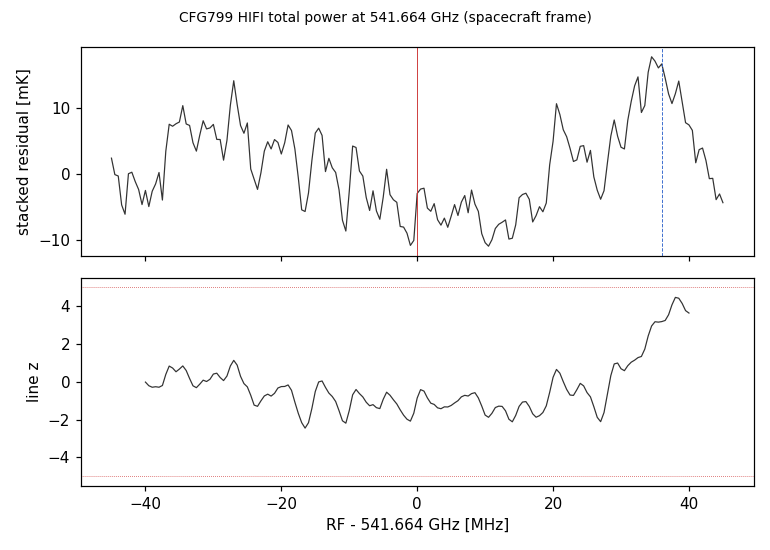
\includegraphics[width=0.72\linewidth]{PAPER53_fig_stack.png}\\
{\footnotesize Stacked total-power residual (top) and line significance (bottom) around 541.664\,GHz, in the spacecraft frame.}
\end{center}

\textbf{Controls (all pass).}
\begin{itemize}
\item Injection recovery: exact. A mismatched profile recovers 0.94.
\item Null offsets at $\pm5$, 10 and 20\,MHz: $p=0.24$.
\item An IF-shuffled stack over 3040 fits is consistent with zero ($z=+0.20$).
\item The Level-1 anchor passes for 53 of 55 observations.
\item A mutation run that injects a 77\,mK line into total power only recovers it at $z=9.1$ and classes it as a line candidate.
\end{itemize}

\textbf{The 541.700\,GHz excess.} The $3.2\sigma$ excess at the secondary frequency is below threshold. It falls in the look-elsewhere region: the largest $|z|$ in a $\pm40$\,MHz scan is 4.45, near the same frequency. It is also within the Doppler range of source lines across epochs. We reported it as a hint only. \emph{Note added in v1.1:} a pre-registered follow-up (lane CFG802) traced it to the instrument. The excess appears only in the H-polarisation receiver ($z=+5.3$) and is absent in V ($z=-0.5$); a field of random polarisation would appear in both. It is also broad, with significance peaking at an assumed FWHM of 4\,MHz rather than the 1.1\,MHz instrument width. The trials-corrected $p$-value is 0.08. We classify it as an H-receiver baseline feature, not a line. In the same follow-up, an injected narrow line was correctly identified as narrow.

\textbf{Per-observation converter test.} A converter-strength line would be 28--2800\,K (DSB peak), far above the noise of any single spectrum. All 48 observations tested individually exclude it at $5\sigma$ for every $S$.

\section{Interpretation}
\begin{itemize}
\item \textbf{The converter window is closed.} It needs $\varepsilon\approx4$--$6\times10^{-9}$, and we exclude $\varepsilon>1.9\times10^{-11}$, a factor $\sim$200 ($\sim$47 even at $S=1000$). CMB spectral-distortion bounds also exclude it ($\varepsilon\lesssim10^{-13}$, provisional) [5,6], but those are indirect: they assume the field existed and coupled in the early universe. The Herschel bound measures the local field directly.
\item \textbf{The framework survives.} It predicts no line. Its falsification level ($\varepsilon\sim10^{-13}$, PAPER52 v1.1 [2]) is a factor of $\sim$190 below this bound.
\item \textbf{The limiting factor.} The stack is limited by baseline structure ($\chi^2_\nu=2.8$), not by receiver noise. A dedicated dish with a stable baseline remains the decisive experiment.
\item \textbf{Novelty.} To our knowledge, this is the first use of archival space-telescope heterodyne data as a dish-antenna search, and the first direct search at 2.2\,meV. Earlier dish searches covered 0.67--0.92\,meV [4].
\end{itemize}

\section{Caveats}
\begin{itemize}
\item The coupling factor $S$, the effective sideband gain (taken as 0.5), the load coupling (taken as 1) and the local density are provisional. The ε limits scale with them.
\item 4.2\,h of spectral-scan data were not used.
\item The target frequency relies on the fitted coefficient $\kappa=\tfrac12$. The alternative footing gives 595.5\,GHz, which has too little archival coverage here.
\end{itemize}

\vspace{4pt}\hrule\vspace{3pt}
{\footnotesize
[1] This programme (public repository): ARGON03, ARGON06; lanes CFG723, CFG795, CFG797, CFG798, CFG799 (frozen criteria, scripts, outputs).
[2] PAPER52, ``A Two-Frequency Sub-Millimetre Dish Search at 542 and 596 GHz'', v1.1, doi:10.5281/zenodo.23404581.
[3] D.~Horns, J.~Jaeckel, A.~Lindner, A.~Lobanov, J.~Redondo, A.~Ringwald, JCAP 04 (2013) 016.
[4] S.~Knirck et al., JCAP 11 (2018) 031.
[5] A.~Caputo, A.~J.~Millar, C.~A.~J.~O'Hare, E.~Vitagliano, PRD 104 (2021) 095029.
[6] B.~Cyr, J.~Chluba et al., MNRAS 535 (2024) 1874.
Herschel is an ESA space observatory with science instruments provided by European-led Principal Investigator consortia and with important participation from NASA. Data from the ESA Herschel Science Archive.
AI assistance: Anthropic's Claude; parallel AI sessions.}
\end{document}
